\section{Explanation complexity, fidelity and addressability}
\label{sec:explanation-results}

This section answers RQ3 and RQ4 (\S\ref{sec:intro-rq}): how does representation change CLASSIX's intrinsic provenance and ExKMC's post hoc fidelity, and which resulting clusters are operationally addressable? The explanation results separate provenance from approximation throughout: CLASSIX exposes how its own observations are aggregated and merged (\S\ref{sec:classix-math}); ExKMC approximates a separately fitted K Means predictor with axis-aligned rules (\S\ref{sec:resampling-explanation}). Their numbers answer different questions about different objects (\S\ref{sec:lit-gap}) and are never combined into one explanation score.

\textbf{Result (CLASSIX provenance).} The selected compact CLASSIX fit produces 131 aggregation groups that merge into two final clusters. The rich fit produces 559 groups and four final states consisting of three clusters and noise. Every exported customer trace contains the visitor identifier, aggregation group, representative row and final cluster. Both exports reproduce the selected full data labels exactly with ARI 1, confirming the trace is a faithful record of the fitted partition rather than a separate approximation of it.

\textbf{Mechanism and interpretation.} Rich CLASSIX needs more than four times as many aggregation groups even though its final nonnoise cluster count rises only from two to three. This follows directly from the staged process in \S\ref{sec:classix-math}: with nine more standardised dimensions contributing to every pairwise distance, fewer customers fall within a fixed aggregation radius $r$ of any one starting point, so more, smaller groups are needed before the merge step consolidates them into clusters. Group count is therefore a measure of local geometric granularity and computational provenance, not of how difficult the resulting clusters are for a person to read or act on — a large group count does not imply a confusing explanation, only a more finely subdivided intermediate trace.

\textbf{Result (ExKMC fidelity).} The main ExKMC comparison fixes $K$ at four for both representations because both primary K Means selections contain four clusters. At the four-leaf budget, both trees use four effective rules with depth 3 and 2.25 conditions per rule. Compact mean training fidelity is 0.9466 and mean held-out fidelity is 0.9448. Rich fidelity is higher at 0.9639 and 0.9650. Across the five splits, compact held-out fidelity ranges from 0.9416 to 0.9480 and rich fidelity ranges from 0.9599 to 0.9697. This is descriptive split variability rather than inferential uncertainty. The close training and test values give no sign of a training-only gain that disappears on held-out customers.

Compact rules use purchase occasion count and purchase recency across all five splits. Rich rules use purchase occasion count, activity span and the number of distinct top categories. Thresholds are exported in original units after reversing the training scaler and logarithmic transform. Named thresholds support direct database style conditions, but they inherit the meaning and missingness limits of the constructed variables.

\begin{figure}[htbp]
\centering
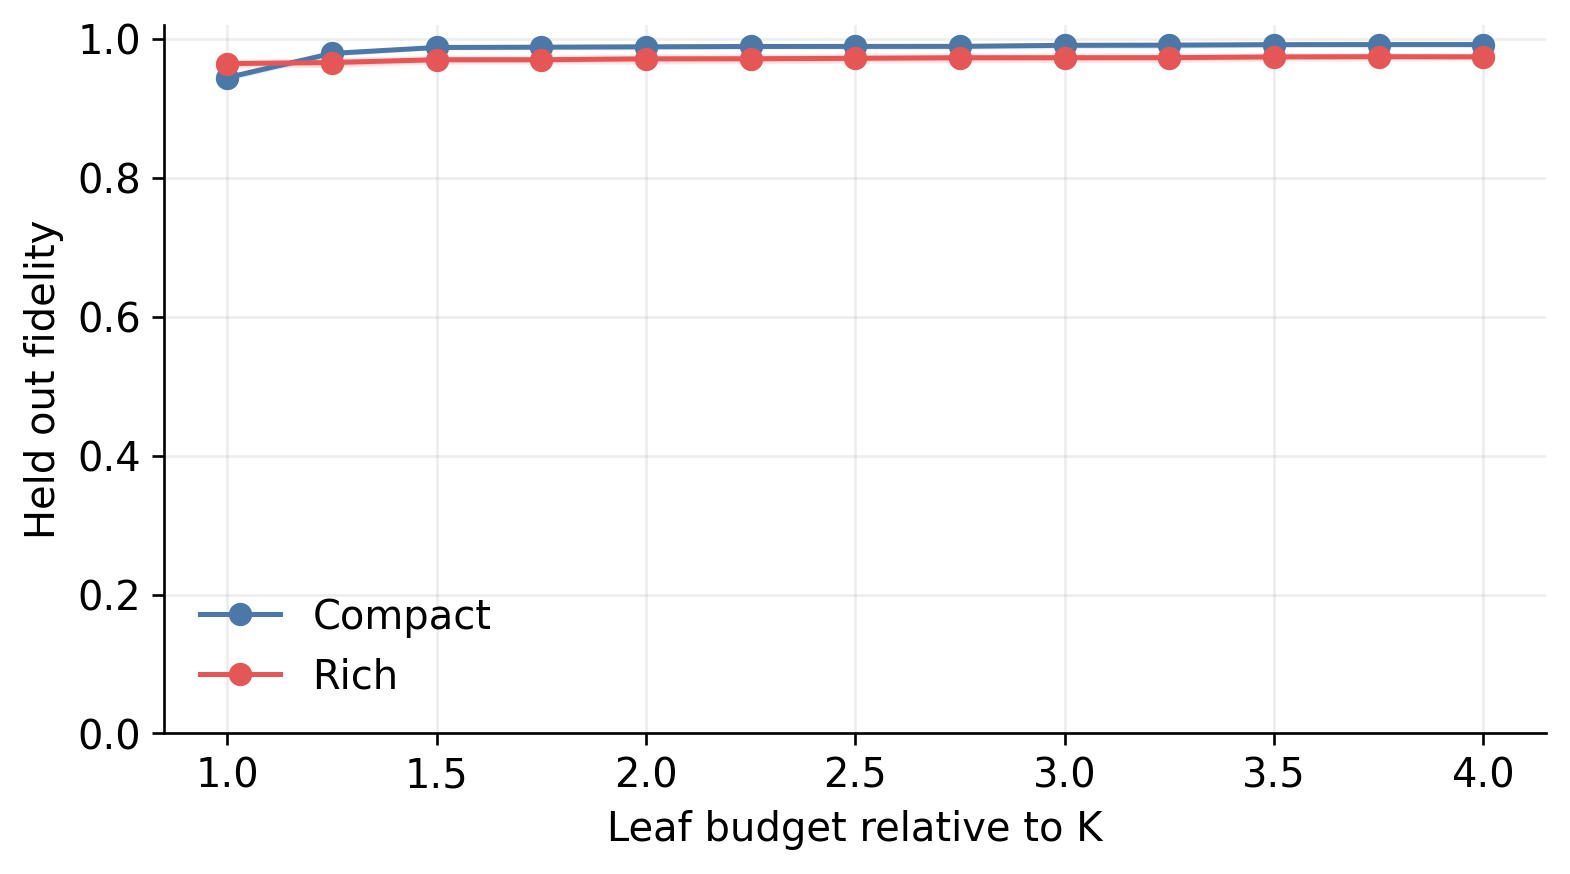
\includegraphics[width=0.75\textwidth]{figures/exkmc_tradeoff.png}
\caption{Held out ExKMC fidelity across the fixed leaf budget}
\label{fig:exkmc_tradeoff}
\end{figure}

Additional leaves change the two fidelity frontiers differently. At sixteen leaves, compact mean held out fidelity reaches 0.9924 with mean depth 6.6 and 4.84 conditions per rule. Rich fidelity begins higher at four leaves but reaches 0.9747 with mean depth 6.4 and 4.74 conditions at sixteen leaves. Compact fidelity begins lower and gains more from expansion. A supplementary training only selection chooses two compact clusters and four rich clusters in every split. Its compact fidelity is 0.9985 with two rules, but that result is not used for the main complexity comparison because $K$ differs.

\textbf{Interpretation.} The crossover between the two fidelity curves — rich ahead at a four-leaf budget, compact ahead by sixteen leaves — shows that representation changes not only \emph{whether} a small tree can approximate K Means well, but the entire \emph{shape} of the complexity/fidelity tradeoff, not merely a single headline number.

\textbf{Limitation.} A higher ExKMC fidelity is evidence that the tree agrees more often with its own K Means reference; per \S\ref{sec:lit-complexity}, it is not evidence that the underlying K Means partition is itself more correct, more useful, or more stable, since fidelity is defined entirely relative to that partition.

\subsection{Addressability: a stricter, distinct criterion}
\label{sec:addressability-hierarchy}

The preceding results show that a cluster can exist, be internally well separated (high silhouette or Calinski--Harabasz), and be highly reproducible under resampling (\S\ref{sec:paired-results}), while still failing to be usable as a targeted business segment. This dissertation therefore treats \emph{addressability} (\S\ref{sec:candidates}) as the last, and strictest, link in a chain of increasingly demanding properties: a partition can \textbf{exist} (any candidate that runs to completion); be \textbf{internally separated} (pass the silhouette/Davies--Bouldin/Calinski--Harabasz validity checks); be \textbf{stable} (survive fixed-parameter overlap-resampling, \S\ref{sec:paired-results}); be \textbf{rule-expressible} (approximated by a short ExKMC tree, or traced by CLASSIX provenance, above); be \textbf{addressable} (pass the size, coverage and distinctiveness audit); and, beyond anything measured in this dissertation, have \textbf{realised business value} (demonstrated to change an intervention outcome). Each property is necessary for the next but not sufficient for it, and this dissertation's evidence stops at addressability.

\textbf{Result.} The addressability audit is stricter than rule export, and most selected clusters fail it despite having already passed the earlier, weaker checks. Neither compact CLASSIX cluster passes because neither differs from the cohort median on at least two named features by the required half interquartile range. In the rich result, the 33-customer cluster is too small, the 1,137-customer cluster has zero category coverage, and the 10,331-customer cluster lacks two sufficiently distinctive median conditions. None of the five nonnoise CLASSIX clusters is classified as addressable. No compact K Means cluster passes. One of four rich K Means clusters passes all gates, while the others fail because they have too many distinguishing conditions or insufficient category coverage.

\textbf{Interpretation.} The compact CLASSIX partition (Table~\ref{tab:customer_results}) has the highest silhouette of any selected configuration in this dissertation, yet zero of its clusters are addressable; the rich K Means partition has the lowest compact-comparison silhouette among the four selected configurations, yet it is the only one to produce an addressable cluster. Internal validity and addressability are evidently not the same property and do not even rank configurations in the same order — a result that could not be seen without evaluating both explicitly.

\textbf{Limitation.} Business interpretation remains narrow at every stage of this hierarchy. Rich features expose a high-activity minority and a group with missing category histories, described here only as observed contrasts in recorded behaviour. ExKMC shows that K Means assignments \emph{can} be represented with a small number of named thresholds at high held-out fidelity; it does not show that a person will find those thresholds meaningful. The one passing rich cluster meets a technical audit rather than an outcome test. The observed value in this dissertation is limited to queryability and auditable coverage — the fifth link in the chain above. Revenue effect, campaign response and human comprehension, the sixth link, remain entirely unmeasured and are not claimed.
